%pygmentize_options: -O startinline=True

\chapter{Analysing PHP Code}

    The PHP programming language first appeared in 1995\cite{phphist}. Over the years 
    the language has involved and so have the ways how programmers were using it. 
    This project focuses on PHP version 5.5\footnote{From this point, 
    if the PHP version is not stated explicitly, it is implicitly 5.5.} 
    and the aim for the analysis 
    is to work well on PHP source code written in an object oriented manner, 
    using modern PHP patterns and idioms that are described later in 
    this text. The analysis, however, should work reasonably good on 
    any valid PHP code. We do not focus only on websites, but also on 
    PHP libraries and frameworks that by themselves do not contain 
    any PHP files that produce HTML or any other output for the user.
    
    \section{PHP semantics}
    This section describes some important parts of the semantics of 
    the PHP programming language, especially those that represent a 
    challenge for static analysis.
    
    \subparagraph*{}    
    In PHP, local or global variables, object fields and function or 
    method parameters are dynamically typed, which means that they 
    can hold values of completely different types at different 
    times of execution.
    
    \subsection{Local Variables}
    Local variables in PHP do not need to be declared explicitly. 
    Instead the first usage of a variable is also its declaration. 
    If a variable's value is used before the variable got any 
    value assigned, then the interpreter generates a notice, 
    however the execution continues and value \code{null} is 
    used instead. A variable can get a value assigned to it when it 
    appears on a left hand side of an assignment or when a 
    reference to that variable is created, in which case it gets value 
    \code{null}. Note: references are discussed in one of the following 
    subsections.

    The scope of a local variable is always its parent function not the 
    parent code block as in other languages like C or Java. So in the following 
    example, the usage of variable \code{\$y} at the end of the function 
    can generate uninitialized variable notice, however, if \code{\$x} 
    was equal to \code{3}, \code{\$y} will have a value although it 
    was declared in the nested code block.

%pygmentize_begin php
% function foo($x) {
%   if ($x == 3) { $y = 2; }
%   echo $y; // uninitialized variable if x != 3
% }
%pygmentize_end
    
    \subsection{Global and Local Scope}

    \subsection{Closures}
    PHP also supports anonymous functions. An anonymous function has its 
    own scope as any other function and its local variables are not visible 
    to the scope where it was declared

    \subsection{Interesting Control Flow Structures}
    \note{Arbitrary expressions in continue and break.}
    
    \subsection{Conditional Declarations}
                
    \subsection{Auto-loading}
    
    \subsection{PHPDoc Annotations}
    
    \section{Static Code Analysis}       
        Static analysis of source code is an analysis that is performed without 
        executing the code. This means that we do not have to have a
        web server for example in order to analyse code of a web application. 
        We can also guarantee some properties that would not be possible to 
        guarantee if we executed the code. Namely the halting property and 
        upper bounds on time and space complexity. Arbitrary code may not 
        halt if executed, but static analysis of such code can still halt 
        and give us some results.
        
        Static analysis can be used to get possible types of an expression in 
        a dynamically typed language, to find out expressions that have constant 
        value through constant propagation and many other problems. 
        Static analyses usually do not give accurate solution, but 
        its approximation, which can be an over-approximation or 
        an under-approximation and it is up to the designer and user of the analysis 
        which one is acceptable for his or her\footnote{``His'' or ``he'' 
        should be read as ``his or her'' or ``he or she'' through the rest of the text.} 
        purposes.                
        
        \subsection{Terminology}
        %More detailed description of what static analysis is 
        %(as opposed to for example explicit model checking, 
        %verification, etc.). Terminology: context sensitive, 
        %path sensitive, symbolic execution, abstract interpretation, etc.                    
        
        Static analyses are usually described in the form of inference rules. 
        An example of an inference rule can be 
        ``if the types of expressions $e_1$ and $e_2$ are integers, then the type of 
        expression $e_1+e_2$ is integer''. Those rules can be more formally 
        described with the following notation        
        $$
        \infer{\vdash e_1+e_2 : Integer}{\vdash e_1 : Integer & \vdash e_2 : Integer}
        $$        
        where above the horizontal line we have hypothesis and below is 
        the conclusion. The exact notation is not important we will be using it 
        intuitively to illustrate the ideas that we describe.
        
        \paragraph{Flow Sensitivity.}
        The example inference rule is not valid, if we admit that evaluation of 
        expression $e_1$ can influence the type of expression $e_2$ or vice versa. 
        In such case, the ordering of the expressions is important, but not captured 
        in the inference rule. Therefore this rule is \emph{flow insensitive}. If we make 
        the hypotheses more complex to capture the ordering 
        it will be \emph{flow sensitive}.
        
        \paragraph{Path Sensitivity.}
        If we admit conditional control flow statements, like if-then-else, 
        we can have more possible paths through the program. In our example, 
        let us say that there is an if statement before the expression $e_1$
        and the expression $e_1$ can evaluate to different 
        type if the then branch of the if-then-else statement is taken than 
        if the else branch is taken. This is illustrated in the following code listing. 
        If the inference rules do not model this, like our example rule, 
        we say that the inference system is 
        \emph{path insensitive}, otherwise we say 
        that it is \emph{path sensitive}.
        
%pygmentize_begin php
% if (...) $x = 3;
% else $x = 'string';
% $e_1 = $x;
% $e_2 = 4;
% $e_1 + $e_2;
%pygmentize_end        
        
        \paragraph{Abstraction.}
        Another example of problem that can be partly solved with static analysis 
        is the sing of integral variables. We can have inference rules of the 
        following form.
        $$
        \infer{\vdash v_1+v_2 : -7 (sign: \ominus)}
        {\vdash v_1 : -10 (sign: \ominus) & \vdash v_2 : 3 (sign: \oplus)}
        $$
        However, the implementation would not be very efficient and we sometimes 
        do not have the full information about variables values, but in some cases 
        we can deduce another useful piece of information by other means. For example, variable of 
        type \code{unsigned integer} will always be positive, we can count on that 
        even if we do not know the actual value. What we 
        can do is to abstract the possible integral values with set 
        $\{0, \ominus, \oplus\}$ with the following meanings         
        \begin{itemize}
            \item $\ominus$ represents all negative integers,
            \item $\oplus$ represents all positive integers,
            \item $0$ represents zero,
        \end{itemize}                
        and rewrite the inference rules as follows:
        $$
        \infer{\vdash v_1+v_2 : \ominus}
        {\vdash v_1 : \ominus & \vdash v_2 : \ominus}
        $$
        Nonetheless, there is another problem. What to do when we have $\ominus$ 
        and $\oplus$ in the hypothesis.
        $$
        \infer{\vdash v_1+v_2 : ?}
        {\vdash v_1 : \ominus & \vdash v_2 : \oplus}
        $$
        The solution is to extend the domain so that it is closed under all operations. 
        We add another element to our set:
        \begin{itemize}
            \item $\top$ represents an unknown value (either positive, negative, or zero).
        \end{itemize}
        Then the rule will be:
        $$
        \infer{\vdash v_1+v_2 : \top}
        {\vdash v_1 : \ominus & \vdash v_2 : \oplus}
        $$
        And for example another rule dealing with $\top$ in hypothesis:
        $$
        \infer{\vdash v_1+v_2 : \top}
        {\vdash v_1 : \ominus & \vdash v_2 : \top}
        $$               
    
        \subsection{Data Flow Analysis}
        Data Flow Analysis (DFA) is a static analysis framework 
        for compiler optimizations and verification that 
        scales to large code bases 
        \cite{nielson1999principles}, \cite{aho1985compilers}.
        
        \paragraph{Control Flow Graph.} 
        DFA is typically performed on a control flow graph, 
        although there are also existing approaches to DFA 
        without explicit control flow graph 
        construction \cite{mohnen2002graph}.
        
        Control flow graph nodes, also called basic blocks, 
        are program statements that are always sequentially executed. 
        Directed edges represent the control flow between basic blocks, 
        i.e. jumps in the control flow due to conditionals, 
        goto statements or any other statements that can change 
        the flow of the program.        
        Control flow graphs usually contain two special nodes: 
        entry node and exit node. Entry node does not have any 
        incoming edges and all the paths lead to the exit node.        
        An example of a control flow graph is given in figure \ref{cfg}.
        
\begin{table}[h]
  \begin{tabular}{ l | m{6cm} }
  \centering
    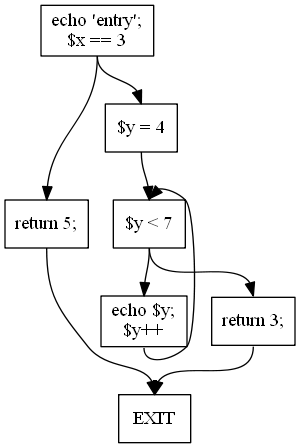
\includegraphics[scale=0.7]{img/cfg.png}
  &
 
\begin{minipage}{6cm}
%pygmentize_begin php
%   echo 'entry';
%   if ($x == 3)
%       $y = 4;
%   else
%       return 5;
%        
%   while ($y < 7) {
%       echo $y;
%       $y++;
%   }
%
%   return 3;
%pygmentize_end
\end{minipage}

  \\
  \end{tabular}
  \caption{Control flow graph\label{cfg}}  
\end{table}          
        
        \paragraph*{Lattices.}
        The reasoning behind correctness and termination of DFA 
        is based on an algebraic structures called lattices. 
        A lattice is a partially ordered set in which every 
        two elements have a least upper bound, called supremum, 
        and a greatest lower bound, called infimum.
        
        \emph{Bounded lattice} is a lattice that has 
        a greatest element and a least element, 
        usually denoted as $\top$ and $\bot$. 
        A bounded lattice is depicted in figure \ref{lattice}.       
        
\begin{figure}[h]  
  \centering
    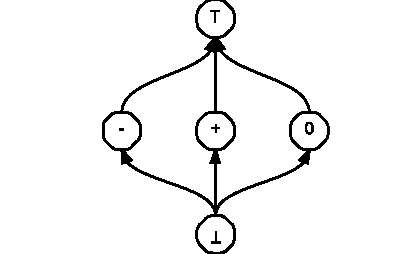
\includegraphics{img/lattice.pdf}
  \caption{Bounded lattice with 5 elements.\label{lattice}}    
\end{figure}

        What is important about lattices for 
        DFA analysis is that if we have a 
        lattice $(S, \leq_{s})$ and a function 
        $f:S\rightarrow{S}$ that is monotonous, 
        i.e. $\forall{a\in{S}}: a\leq_s{f(a)}$, then 
        $f$ has a fixpoint. That is a point $x\in{S}$ for 
        which $f(x)=x$.
        
        Intuitively, $f$ has to have a fixpoint because 
        for every argument $y$, it must either return 
        $y$ itself, but then $y$ is a fixpoint, or it 
        returns an element that is greater than $y$, 
        but this cannot go on forever, because eventually 
        $f$ will be given $\top$ for which it does not have 
        any other option but returning $\top$ and we 
        have a fixpoint again.
        
        
        \paragraph*{}
        \note{The following few paragraphs will finish the description 
        of Data Flow Analysis.}

        \subsection{Intraprocedural Analysis}
        So far we have been discussing an analysis of a 
        single function or method\footnote{We will use term 
        routine to designate a function, static or instance method}. 
        However, if we want to analyse whole program or 
        a library, the interaction between the routines 
        can be takend into account to make it more precise.
        
        \paragraph{Context Sensitive Intraprocedural Analysis.}
        The most precise solution would be take into account 
        the calling context when analysing a function. 
        In different contexts, the function can be, 
        for example, given different parameters values 
        which may then influence the result of the analysis. 
        More precise result for a specific call site context 
        can be propagated to that call site, 
        yielding another gain in precision when 
        analysing the function that realises the call.
        
        \paragraph*{}
        \note{The following few paragraphs will discuss 
        feasibility of Context Sensitive Intraprocedural Analysis, 
        because call sites are not always known, 
        practical consequences and usual approaches to 
        make Context Sensitive Intraprocedural Analysis 
        more scalable.}
    
    \section{Control Flow for Phalanger Approach}
        \note{Description of the analysis used in our case using the terminology 
        built up in the previous section. It will be more 
        abstract description, without technical details 
        about implementation.}